\section{MapReduce}
\subsection{Présentation et fonctionnement}

\par MapReduce est un patron d'architecture de développement informatique, inventé par Google. Un de ses principaux objectifs est de réaliser des calculs parallèles et souvent distribués sur des jeux de données très volumineuses (de l'ordre du téraoctet, voire du pétaoctet). Compte tenu la volumétrie des données mises en jeu, il devient inconcevable de réaliser des traitements au cas par cas. La particularité de MapReduce réside en ce que le développeur Hadoop prend en considération qu'un seul enregistrement. La généralisation à l'ensemble des données est gérée par Hadoop.

\par Le fonctionnement de MapReduce se décompose en trois parties :
\begin{itemize}
\item le \textit{driver} s'exécutant chargé de configurer le job et de le soumettre pour exécution;
\item le \texttt{mapper} chargé de lire les données dans le HDFS et de les traiter;
\item le \texttt{reducer} chargé de consolider les résultats issus du \texttt{mapper} et de les écrire sur le HDFS. L'utilisateur peut ensuite les récupérer sur son disque local.
\end{itemize}

\par De manière très schématique, un programme MapReduce comporte toujours deux fonctions : \textit{map} et \textit{reduce} (cf. figure~\ref{fig:mapreduce-exp}). La première a pour tâche de parser les données présentes en entrée en un ensemble de paires \texttt{<clé, valeur>} envoyées en entrée de la fonction \textit{reduce} où \texttt{clé} et \texttt{valeur} sont entièrement définies par le développeur en fonction des besoins. Cette dernière se charge de la réduction des paires selon la \texttt{clé}. Il est essentiel d'avoir à l'esprit la spécialisation des n\oe{}uds esclaves en noeuds exécutant des fonctions \textit{map} ou des fonctions \textit{reduce} uniquement.

\begin{figure}[h!]
  \centering
  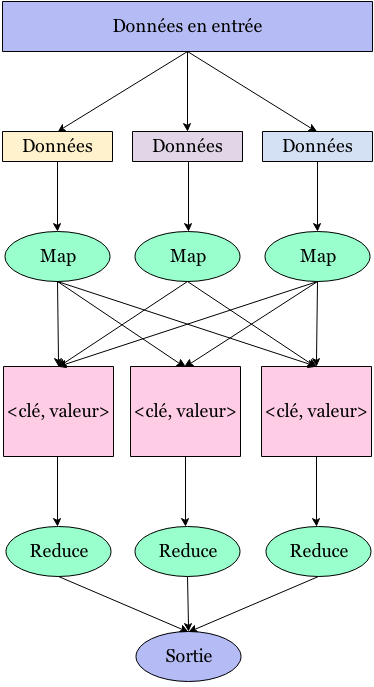
\includegraphics[scale=0.4]{images/mapreduce_arch.png}
  \caption{Architecture du patron MapReduce}
  \label{fig:mapreduce-exp}
\end{figure}

\par L'architecture Hadoop est développée dans le but de traiter une volumétrie de données très conséquente. Or il est clair qu'un facteur de ralentissement de traitement réside dans la transmission des données (lecture/écriture). Par conséquent, Hadoop esquive au plus cette limitation technologique en envoyant le code MapReduce dans les DataNodes où les données ont au préalable été transférées. Ce ne sont plus les données mais le code qui transite désormais, et ce à quelque exception près que nous détaillons ci-dessous.

\subsection{Shuffle \& Sort}

\paragraph{Les phases de \textit{shuffle} et \textit{sort}.} La synchronisation des fonctions \textit{map} et \textit{reduce} est rendue possible par des processus supplémentaires : \textit{shuffle} et \textit{sort}. \textit{sort} tri les jeux \texttt{<clé, valeur>} par \texttt{clé}. \textit{shuffle} est le processus permettant de réaliser le \textit{sort} et de transférer les données en sortie des \textit{map} vers l'entrée des \textit{reduce}. On comprend donc l'utilité de tels processus couplé à la spécialisation des n\oe{}uds esclaves. Par conséquent, le processus \textit{shuffle} est la base de MapReduce et c'est dans celui-ci que la magie s'opère.

\paragraph{La fonction \textit{map}.} Cette fonction ne se réduit pas simplement à la transformation des données sous le format mentionné et à son écriture sur le disque mais est bien plus complexe. Le processus en question s'appuie sur le tampon mémoire du n\oe{}ud esclave où sont écrit les données au fur et à mesure (en \textit{streaming}) tout en les pré-triant pour des raisons de performance. La figure~\ref{fig:shuffle-sort-mapred} détaille ce qui se passe.

\begin{figure}[h!]
  \centering
  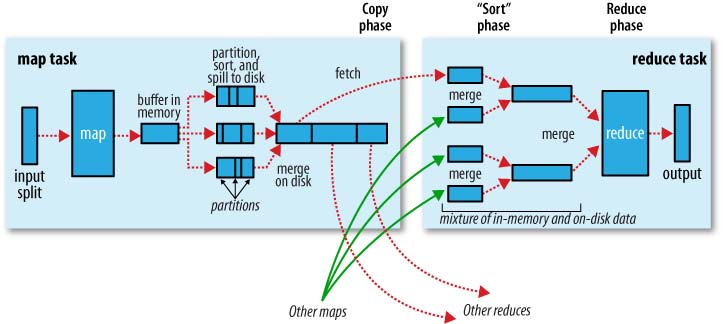
\includegraphics[scale=0.6]{images/shuffle_sort_mapred.png}
  \caption{\textit{shuffle} et \textit{sort} dans MapReduce. \\Source : O'Reilly | Hadoop: The Definitive Guide}
  \label{fig:shuffle-sort-mapred}
\end{figure}

\par Chaque \textit{map} possède un buffer circulaire dans lequel celui-ci écrit les données en sortie. Sa taille par défaut est de 100MB mais peut être modifiée à l'aide de la propriété \texttt{io.sort.mb}. Lorsque le contenu du buffer atteint un certain seuil (par défaut : 80\% paramétrable avec \texttt{io.sort.spill.percent}), un thread est lancé en fond chargé de transférer le contenu du buffer dans le disque du n\oe{}ud. Par abus de langage, ce thread peut être appelé : \textit{spill} (c'est le terme anglais désignant l'opération réalisée). Ainsi, les données en sortie du \textit{map} vont continuellement être écrites dans le buffer jusqu'à ce que le \textit{spill} soit lancé. Le cas de blocage de la fonction \textit{map} apparaît lorsque le buffer se remplit. Dans ce cas, la fonction \textit{map} attend que le thread \textit{spill} le vide pour continuer.

\par Cependant, avant d'écrire les données sur le disque, celles-ci sont partitionnées selon les \textit{maper} vers lesquelles elles seront envoyés par la suite. Chaque partition est ensuite triée ce qui permettra d'accélérer le \textit{reducer}. Remarquons que plusieurs threads \textit{spill} peuvent être créés. En effet, rien n'empêche d'atteindre le seuil après la création d'un thread en ce que l'opération \textit{map} peut être plus rapide que le thread. Ce raisonnement nous amène à considérer l'existence de plusieurs threads et nous comprenons qu'à chaque création d'un thread il devient de plus en plus difficile d'atteindre à nouveau le seuil.

\par Avant la fin de la fonction \textit{map}, l'ensemble des partitions est regroupé (\textit{merge}) en une seule et même partition triée par clé et prête à être envoyée à un \textit{reducer}. Les partitions en sortie des \textit{maper} sont ensuite acheminées vers les  \textit{reducers} par le biais du protocole HTTP.

\paragraph{La fonction \textit{reduce}} Cette fonction prend en entrée les sorties des différentes \textit{maps}. Ces dernières peuvent se terminer à des instants différents les unes des autres; instant pouvant varier en fonction du matériel utilisé et des données stockées. Ainsi, le les \textit{reducers} commencent à copier les données en \textit{streaming}. C'est la phase de copiage réalisée par plusieurs threads du \textit{reducer} qui vont recopier les données en parallèle. La valeur par défaut est cinq mais reste paramétrable.

\par Maintenant il est question de connaître les données en sortie des \textit{maps} que le \textit{reducer} doit copier. Pour ce faire, au fur et à mesure de l'exécution du job au sein des n\oe{}uds \textit{map} des signaux d'état (\textit{heartbeat}) sont envoyés aux noeuds maîtres qui sont le JobTracker (Hadoop 1.x) ou le ResourceManager (Hadoop 2.x). A leur tour ils renseignent aux \textit{reducers} l'emplacement des données à copier. Les données stockées dans les \textit{mapers} ne sont effacées qu'à la fin du job et ce afin de pallier à une quelconque panne.

\par Les données recueillies sont regroupées au fur et à mesure en partitions de taille définies. Lorsque la phase de copiage (\textit{copying phase}) est terminée et qu'un certain nombre de tailles définies ont été créés, la phase de trie (\textit{sort phase}) démarre.

\par L'invocation de la fonction \textit{reduce} pour chaque clé sur les données réorganisées et triées marque le début de la phase de réduction (\textit{reduce phase}). Le pré-tri réalisé dans les étapes précédentes prend tout son intérêt ici. En effet, l'ensemble des \texttt{valeurs} associées à une certaine \texttt{clé} se trouvent à la suite. La fonction \textit{reduce} est par conséquent optimisée en ce qu'elle s'épargne un tri pouvant s'exécuter sur des millions de paires. La sortie de cette phase est écrit  directement sur HDFS. L'utilisateur est ensuite en mesure de récupérer les données.


%\par La figure~\ref{fig:mapreduce-exp} donne l'aperçu global du patron MapReduce. Les données présentées en entrée sont splittées. Concrètement, les données splittées correspondent tout simplement aux blocs stockés dans les DataNodes des fichiers (cf \ref{sec:hdfs}). C'est sur ces données que va s'exécuter la fonction \textit{map} dans un premier lieu. La particularité c'est que c'est le code qui est envoyé sur les noeuds esclaves et non les données qui y sont déjà présentes. En terme d'I/O, les performances de calculs sont considérablement augmentées puisqu'on s'épargne le temps de transfert des données.
%
%\par Plusieurs fonctions \textit{map} peuvent s'exécuter simultanément. Ceci est possible du fait de l'architecture maître-esclave. La parallélisation des calculs augmente donc le temps de traitement.
%
%\subsection{Les I/O}
%\label{sec:mapreduce-io}
%
%\par Dans un algorithme MapReduce, les données présentes en entrée/sortie des tâches \textit{map} et \textit{reduce} sont toujours sous la forme \texttt{<key, value>} ou \texttt{<clé, valeur>}. Imposer cette structure unique et simple aux enregistrements contribue à l'efficacité d'Hadoop au niveau des I/O.
%
%\subsection{La fonction \textit{map}}
%
%\par Le programme le plus simple permettant de comprendre le patron MapReduce est le \texttt{wordcount}. Celui-ci permet de compter le nombre d'occurrences des mots d'un ou plusieurs fichiers. Afin d'illustrer la fonction nous prenons cet exemple. Le code source Java ainsi que les \texttt{input} et \texttt{output} sont joints à ce rapport.
%
%\paragraph{Le << parsage >> des données.} Un fichier texte en entrée de la fonction \textit{map} est traitée de façon très spécifique. En effet, la fonction \textit{map} prend en entrée une ligne du fichier. Le fichier ci-dessous
%
%\begin{quote}
%banane wiki mangue mac toto\\
%mac kiwi galaxy banane kiwi\\
%\end{quote}
%
%présenté en entrée de la fonction \textit{map} du \texttt{wordcount} produira le jeu de <clé, valeur> suivant :\\
%
%\centerline{
%\begin{tabular}{|c|c|}
%\hline  1ère phrase & 2ème phrase \\ 
%\hline banane, 1 & mac, 1\\wiki, 1 & kiwi, 1\\ mangue, 1 & galaxy, 1\\ mac, 1 & banane, 1\\ toto, 1 & kiwi, 1\\
%\hline 
%\end{tabular}} 
%
%\subsection{La fonction \textit{reduce}}

%%% Local Variables: 
%%% mode: latex
%%% TeX-master: "CompteRendu"
%%% End: 